\chapter{Результаты}

Мною была написана программа, реализующую натурную модель с 
базовой топологией с двумя хостами и одним коммутатором для реализации
программы.
 
Полная реализация программы приведена в разделе \textbf{Приложения},
для вывода графиков была использована программа GNUPLOT.

Смоделировал сеть три раза с указанными параметрами. В первом случае добавили задержку в 100 мс на обоих хостах, во втором случае 50мс, в третем случае 100мс с отклонением в 10мс и запустив gnuplot-скрипт, я получил следующий график(рис.~\ref{fig:3.1}).

\begin{figure}[!ht]
  \centering
  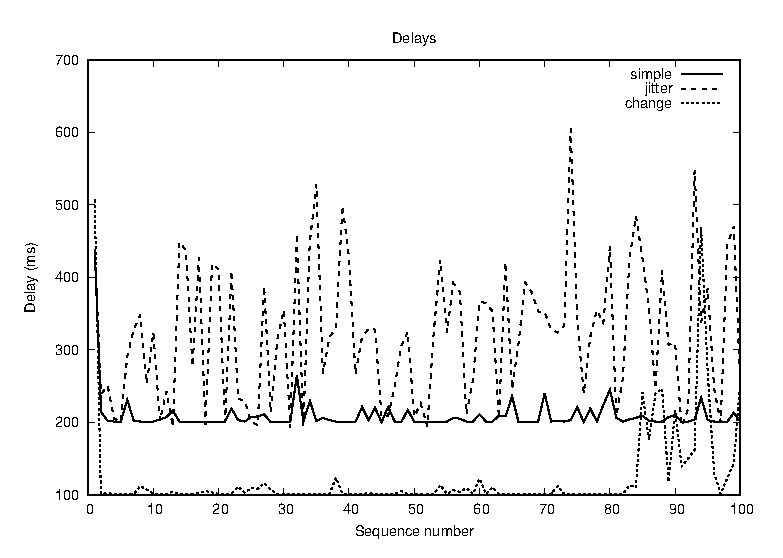
\includegraphics[width=0.6\linewidth]{image/pings.eps}
  \caption{Измерение задержек при разных условиях}
  \label{fig:3.1}
\end{figure}

Как мы видим из графика, наименьшие задержки имеет сеть с задержкой в 50 мс, при указании отклонения в 10мс задержки возрастают в несколько раз.


На коммутаторе s1 указал дисциплину очереди red со следующими параметрами: минимальный порог сброса в 30000 байтов, максимальный в 60000 байтов.
Смоделировал сеть и с помощью iperf3 получил графики окна перегрузки, пропускной способности и количества переданных байтов. Изменил дисциплину очереди c red на ared. Вывел соответствующие графики также и для этой модификации (рис.~\ref{fig:3.2}, \ref{fig:3.3}, \ref{fig:3.4}, \ref{fig:3.5}, \ref{fig:3.6}, \ref{fig:3.7}).

\begin{figure}[!ht]
  \centering
  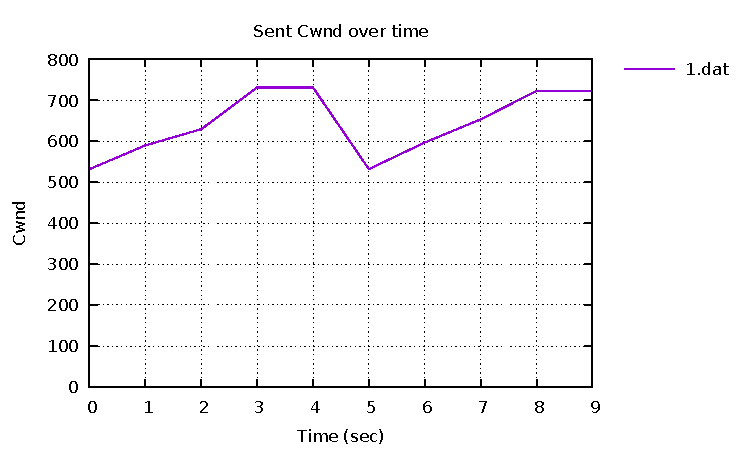
\includegraphics[width=0.6\linewidth]{image/red/cwnd_red.pdf}
  \caption{Окно перегрузки при использовании red}
  \label{fig:3.2}
\end{figure}

\begin{figure}[!ht]
  \centering
  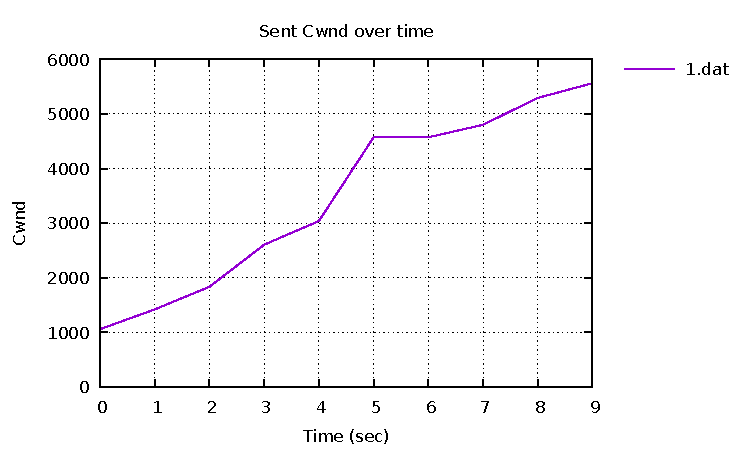
\includegraphics[width=0.6\linewidth]{image/ared/cwnd_ared.pdf}
  \caption{Окно перегрузки при использовании ared}
  \label{fig:3.3}
\end{figure}

Как мы видим, при классическом алгоритме размер TCP окна перегрузки значительно меньше. 


\begin{figure}[!ht]
  \centering
  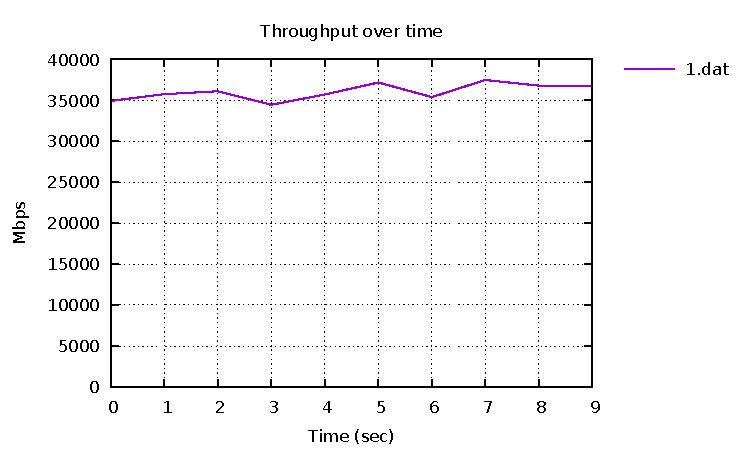
\includegraphics[width=0.6\linewidth]{image/red/throughput_red.pdf}
  \caption{Пропускная способность при использовании red}
  \label{fig:3.4}
\end{figure}

\begin{figure}[!ht]
  \centering
  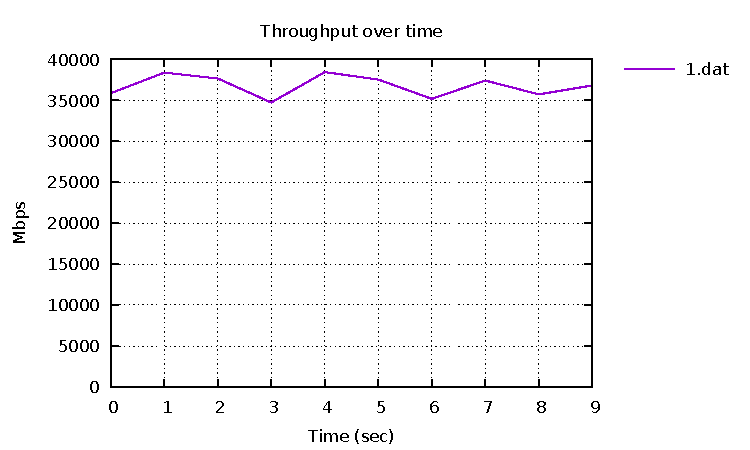
\includegraphics[width=0.6\linewidth]{image/ared/throughput_ared.pdf}
  \caption{Пропускная способность при использовании ared}
  \label{fig:3.5}
\end{figure}

Сравнивая графики пропусеной способности, мы видим, что  adaptive red имеет в среднем немного большую пропускную способность. 

\begin{figure}[!ht]
  \centering
  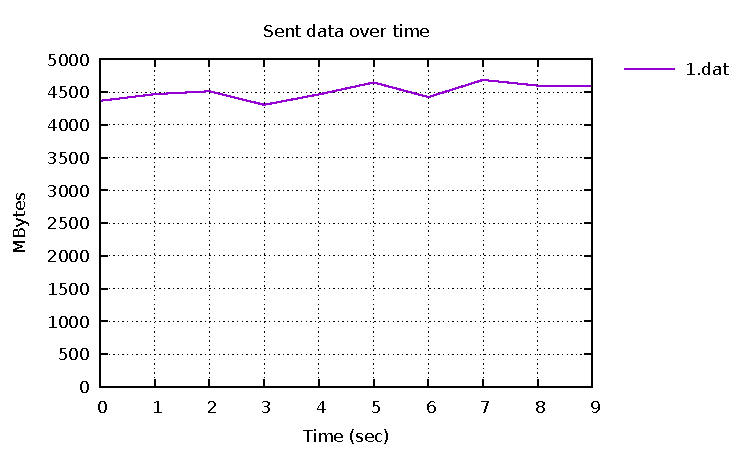
\includegraphics[width=0.6\linewidth]{image/red/bytes_red.pdf}
  \caption{Количество переданных данных при использовании red}
  \label{fig:3.6}
\end{figure}

\begin{figure}[!ht]
  \centering
  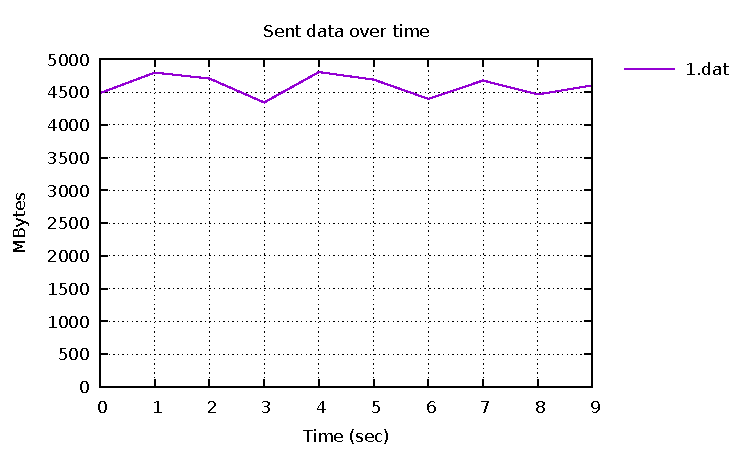
\includegraphics[width=0.6\linewidth]{image/ared/bytes_ared.pdf}
  \caption{Количество переданных данных при использовании ared}
  \label{fig:3.7}
\end{figure}

При ARED также имеем большее количество переданных байтов. 


